\documentclass[10pt,a4paper]{article}
\usepackage[margin=20mm]{geometry}
\usepackage[T1]{fontenc}
\usepackage{lmodern,booktabs,graphicx,amsmath,microtype,xcolor}
\usepackage[colorlinks=true,urlcolor=blue,citecolor=blue,linkcolor=blue]{hyperref}
\graphicspath{{figures/}}
\setlength{\parindent}{0pt}\setlength{\parskip}{5pt}
\title{Small-Model Adaptation on a T4:\\LoRA Quality and Inference Performance of Pythia-410M}
\author{Yash Dave}\date{21 September 2026}
\begin{document}\maketitle
\begin{abstract}
We fine-tune Pythia-410M on a curated mixture of 11 text datasets using LoRA and evaluate quality and inference cost on a Colab Tesla T4. Three main configurations compare ranks 8 and 16 and peak learning rates of $10^{-4}$ and $5\times10^{-4}$. The validation-selected rank-16 adapter reduces held-out test perplexity from 23.1134 to 19.6587 (14.95\%) across 244,760 prediction targets, with improvements on all 11 sources. A 72-case benchmark varies adapter, batch size, precision and prompt length. Batching improves aggregate throughput; FP16 autocast is slower than FP32 in this measured implementation. Results characterize one seed and a small prompt sample, not a universal precision or hyperparameter optimum.
\end{abstract}
\section{Methodology and data}
Pythia is a standard autoregressive GPT-NeoX model family~\cite{pythia}. We use \texttt{EleutherAI/pythia-410m} at revision \texttt{9879c9b5f8bea9051dcb0e68dff21493d67e9d4f}. The model has 24 layers, hidden size 1,024, 16 attention heads, a 4,096-dimensional feed-forward layer and a 2,048-token context capacity. The base has approximately 405.3 million parameters. Training here uses 256-token chunks.

The mixture contains WikiText-2 raw, TinyStories, AG News, IMDb, Yelp Review Full, Amazon Polarity, CNN/DailyMail 3.0.0, XSum, SQuAD contexts, Emotion and Rotten Tomatoes. We use only natural-language fields: articles/documents for news, context for SQuAD, title plus content for Amazon, and text elsewhere. Labels and question-answer targets are excluded. These are sampled corpora, not complete Hub datasets. Exact dataset IDs, subsets and source revisions are in the repository configuration and data manifest.

Preprocessing normalizes Unicode and whitespace, retains 40--20,000-character documents, and deduplicates canonical text. Seeded hash assignment uses 80/10/10 probabilities; per-source caps subsequently retain 1,000/100/100 documents. The retained proportions therefore differ from 80/10/10. Bounded streaming shuffle is practical sampling, not uniform sampling of each entire source. No reasoning-oriented dataset was selected, but content is not semantically screened for every incidental reasoning passage.

\begin{center}\begin{tabular}{lrrr}\toprule
Split & Documents & Chunks & Prediction targets\\\midrule
Train & 11,000 & 16,381 & 2,467,818\\
Validation & 1,100 & 1,634 & 246,145\\
Test & 1,100 & 1,629 & 244,760\\\bottomrule
\end{tabular}\end{center}
Tokenization preserves full documents and appends EOS. Length-256 chunking overlaps one context token, preserving each next-token target exactly once without joining documents. Padding labels are masked by position; genuine EOS targets remain included. Manifests record checksums. Exact deduplication does not rule out near-duplicates or overlap with model pretraining.
\newpage
\section{LoRA training and model selection}
LoRA learns low-rank updates while freezing base weights~\cite{lora}. We target each layer's fused \texttt{query\_key\_value} projection, with dropout 0.05 and no trainable bias. Rank 8 uses $\alpha=16$ and 786,432 trainable parameters; rank 16 uses $\alpha=32$ and 1,572,864. Thus $\alpha/r=2$ is held constant.

All main experiments use AdamW, weight decay 0.01, gradient clipping at 1.0, seed 42, batch size 2 and accumulation 8 (16 chunks per update). FP16 autocast operates over FP32 stored weights with gradient checkpointing. Cosine scheduling follows 154 warmup updates (ceiling of $0.05\times3072$). The common cap is 3,072 updates, approximately three epochs. Validation and checkpoint saving occur every 100 updates and at the end.

Early stopping allows five evaluations without an accumulated improvement of at least 0.001 from the last significant best validation token loss. Absolute best-checkpoint selection is tracked separately, so a run can stop while still making smaller improvements. Rank 16 at $10^{-4}$ stopped at 3,000 updates; the others reached the cap. Colab interruptions were recovered from persistent checkpoints; they are environment interruptions, not evidence of failed hyperparameters. Each resumed execution has its own W\&B segment.

\begin{center}\begin{tabular}{lrrrr}\toprule
Configuration & Peak LR & Stop step & Best step & Val. PPL\\\midrule
Pretrained base & --- & --- & --- & 22.3108\\
Rank 8 & $10^{-4}$ & 3,072 & 2,800 & 19.4830\\
Rank 16 & $10^{-4}$ & 3,000 & 3,000 & 19.2827\\
Rank 16 & $5\times10^{-4}$ & 3,072 & 3,072 & \textbf{19.0935}\\\bottomrule
\end{tabular}\end{center}
\begin{center}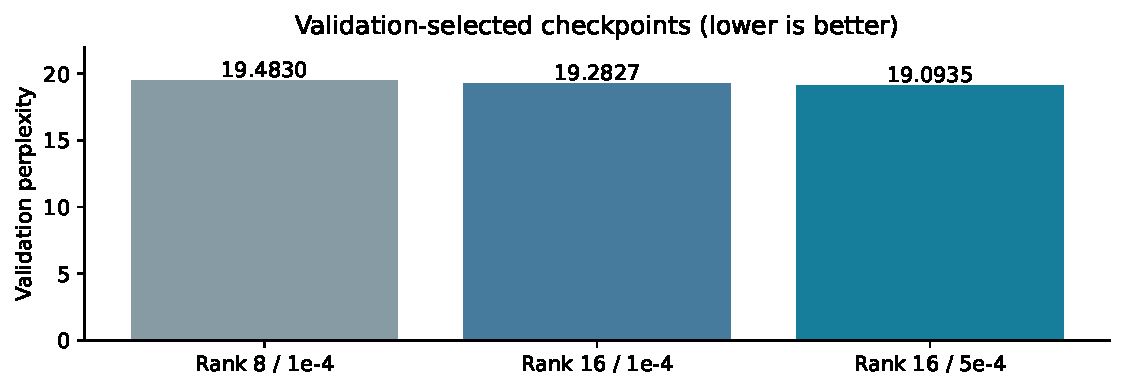
\includegraphics[width=.85\linewidth]{validation_comparison.pdf}\end{center}
The higher learning rate improved rank-16 validation perplexity by approximately 0.98\% relative to $10^{-4}$. This supports selecting it among the tested settings, not claiming an optimal learning rate. The late plateau occurred under a decaying learning rate and does not establish global convergence. A preliminary 300-step rank-8 run was a separate short schedule and is excluded from the main budget comparison.

Token loss is total natural-log negative log-likelihood divided by valid targets. Perplexity is $\exp(\mathrm{loss})$ and bits/token is $\mathrm{loss}/\ln 2$. Sequence loss is summed NLL divided by chunk count and depends on chunk length. W\&B records training loss, throughput, schedule, gradient norm, configuration and checkpoints, plus validation metrics, length buckets, examples and rankings. Final figures are regenerated from saved metrics rather than screenshots.
\newpage
\section{Held-out test results}
We select rank 16 at $5\times10^{-4}$, step 3,072, using validation alone, then compare it with the base on the held-out test split. Both evaluations use identical targets, length 256, batch 2 and FP16 autocast. Other adapters are not retuned on test data.
\begin{center}\begin{tabular}{lrr}\toprule
Metric & Base & Selected adapter\\\midrule
Token loss & 3.140413 & 2.978518\\
Perplexity & 23.113408 & 19.658658\\
Bits/token & 4.530658 & 4.297093\\
Sequence loss & 471.852339 & 447.527333\\\bottomrule
\end{tabular}\end{center}
The test perplexity reduction is \textbf{14.95\%}. All 11 sources improve, although the effect varies substantially. These are next-token language-modeling scores, including for corpora originally built for classification; they do not measure classification accuracy.
\begin{center}\small\begin{tabular}{lrrrr}\toprule
Source & Targets & Base PPL & Adapter PPL & Reduction (\%)\\\midrule
WikiText & 13,848 & 30.595 & 20.801 & 32.01\\
TinyStories & 23,485 & 8.328 & 5.562 & 33.22\\
AG News & 6,176 & 36.090 & 22.375 & 38.00\\
IMDb & 28,411 & 35.365 & 33.585 & 5.03\\
Yelp & 18,117 & 29.284 & 25.875 & 11.64\\
Amazon polarity & 9,943 & 37.515 & 34.071 & 9.18\\
CNN/DailyMail & 77,765 & 22.232 & 19.762 & 11.11\\
XSum & 46,780 & 19.918 & 18.598 & 6.63\\
SQuAD contexts & 15,317 & 20.870 & 20.102 & 3.68\\
Emotion & 2,323 & 103.194 & 45.466 & 55.94\\
Rotten Tomatoes & 2,595 & 117.648 & 47.846 & 59.33\\
\bottomrule\end{tabular}\end{center}
\begin{center}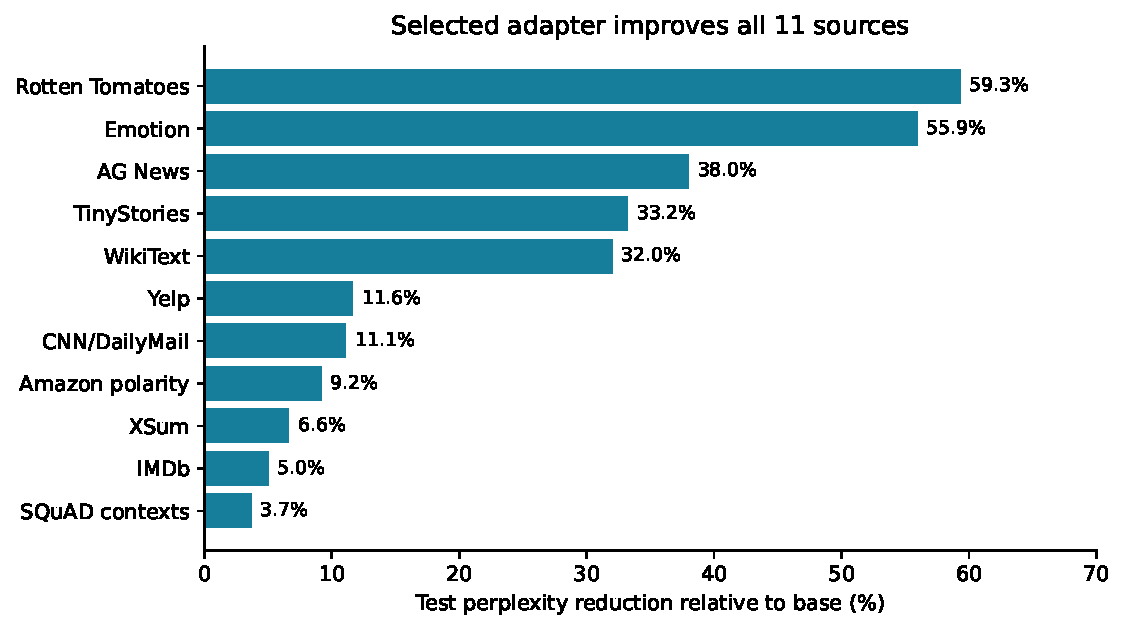
\includegraphics[width=.86\linewidth,height=7cm,keepaspectratio]{test_by_dataset.pdf}\end{center}
Aggregate perplexity is computed from token-weighted loss, not the average of source perplexities. CNN/DailyMail and XSum contribute 50.89\% of test targets despite equal document caps per source. Short-text corpora show larger relative improvements; differences in text and length prevent a controlled causal attribution.
\newpage
\section{Inference benchmark protocol and results}
The benchmark covers four variants (base and the three best adapters), batch sizes 1/2/4, prompt lengths 64/128/256 and FP32/FP16 autocast: 72 cases. Every case completed two warmups and five timed repetitions, totaling 360 measured generations. Each sequence generates exactly 64 tokens using greedy decoding with EOS stopping disabled. Validation-derived prompts avoid test-based benchmark selection; only four source documents are reused across lengths, limiting workload diversity.

Weights remain FP32 in both precision modes. Adapters are \emph{unmerged}; SDPA and KV caching are enabled and TF32 is disabled. GPU-synchronized latency covers full batch generation (prefill plus decoding). Model loading, tokenization, transfers, warmups and logging are excluded. Throughput is total generated tokens divided by total timed seconds, not prompt tokens. Time to first token was not measured. Memory is peak PyTorch allocation/reservation, not total device memory.
\begin{center}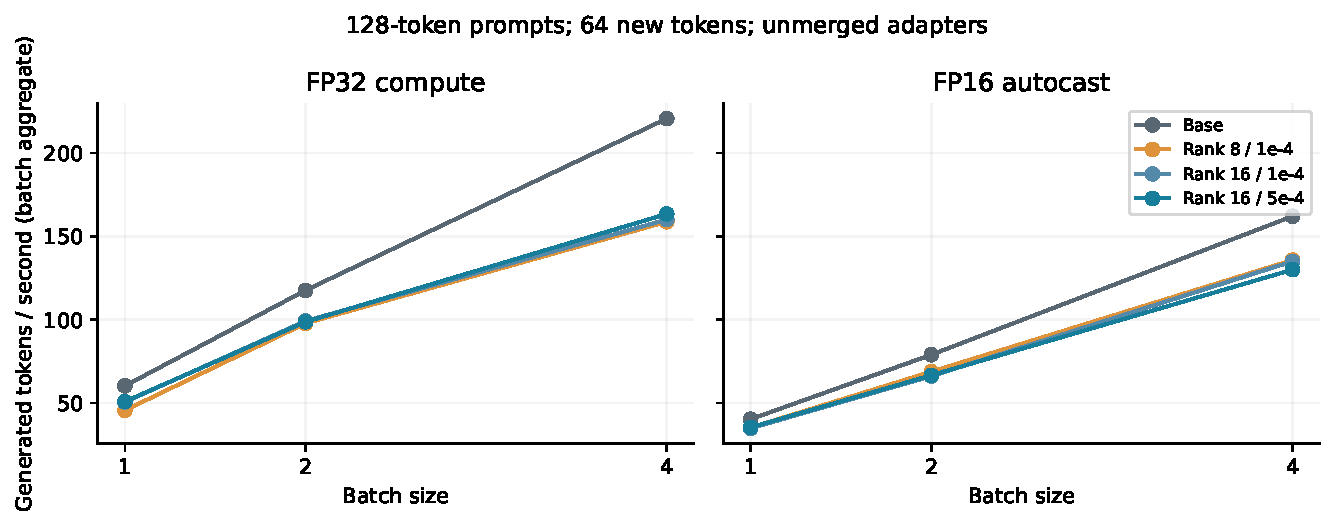
\includegraphics[width=\linewidth]{throughput_by_batch.pdf}\end{center}
At prompt length 128, FP32 base throughput rises from 60.27 to 220.53 tokens/s as batch size increases from 1 to 4. The selected adapter rises from 50.82 to 163.36 tokens/s. This is aggregate throughput: more tokens are generated concurrently, rather than each user necessarily receiving a lower latency.
\begin{center}\small\begin{tabular}{llrrr}\toprule
Variant & Mode & Batch & Latency (ms) & Tokens/s\\\midrule
Base & FP32 & 1 & 1,062.0 & 60.27\\
Selected & FP32 & 1 & 1,259.4 & 50.82\\
Base & FP16 autocast & 1 & 1,588.1 & 40.30\\
Selected & FP16 autocast & 1 & 1,808.0 & 35.40\\
Base & FP32 & 4 & 1,160.8 & 220.53\\
Selected & FP32 & 4 & 1,567.1 & 163.36\\\bottomrule
\end{tabular}\end{center}
FP16 autocast is slower in these measurements. Possible contributors include casting and small-workload launch overhead, but the benchmark does not isolate their causes. Since stored weights remain FP32, these results do not compare fully FP16-loaded versus FP32-loaded models. Rank-8 timing is not consistently faster than rank-16 timing; repeated trials across sessions are needed before attributing small differences to rank.
\newpage
\section{Latency, memory and context-length effects}
\begin{center}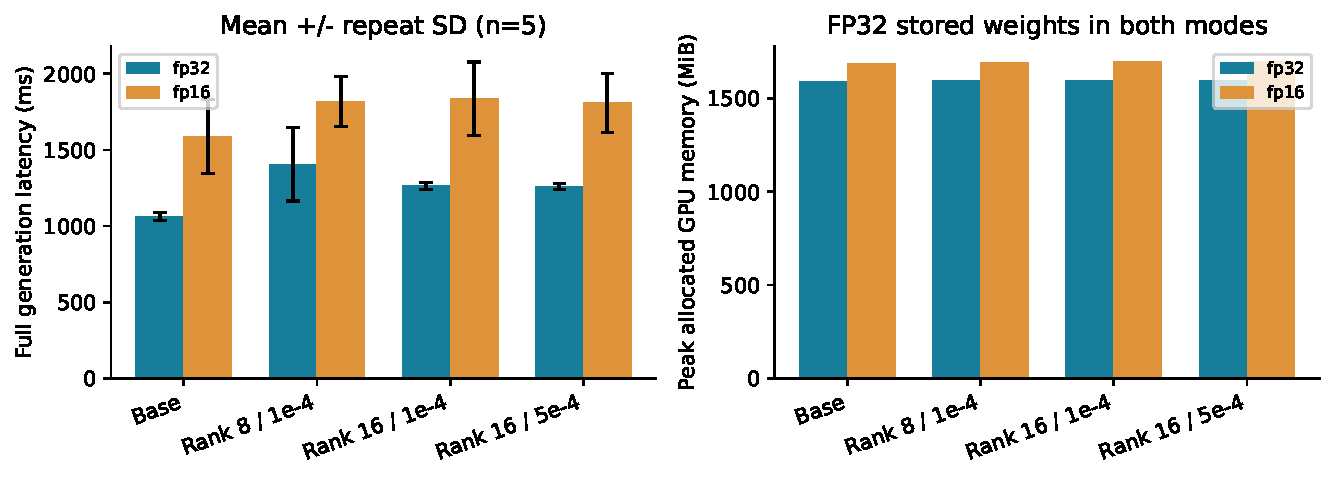
\includegraphics[width=\linewidth]{latency_memory.pdf}\end{center}
At batch 1 and prompt length 128, the selected adapter's peak allocation is approximately 1,598.8 MiB in FP32 and 1,695.9 MiB under FP16 autocast. Keeping FP32 parameters while using autocast can retain additional temporary representations; lower arithmetic precision does not guarantee lower measured allocation for this implementation. Error bars represent the sample standard deviation of five timing repetitions, not confidence intervals or independent training runs.
\begin{center}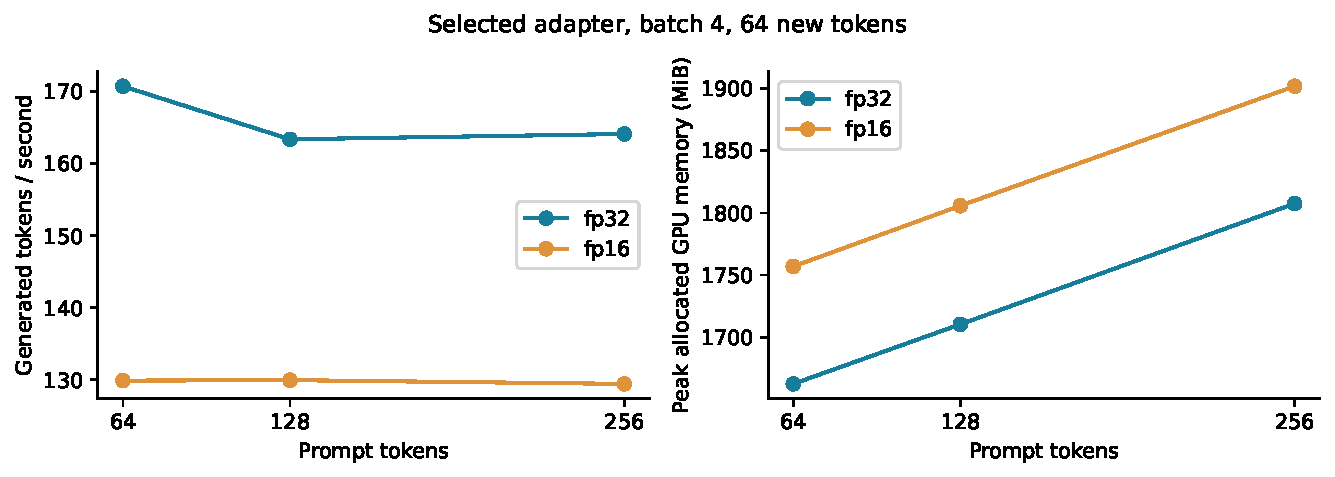
\includegraphics[width=\linewidth]{prompt_length.pdf}\end{center}
These length comparisons vary inference prompts while holding output length fixed. They do \emph{not} compare models trained with different sequence lengths. The repository's sequence-1024 placeholder is not a completed experiment. Full case-level means, repeat timings and allocated/reserved peaks are included in the accompanying JSON/CSV artifacts.
\section{Discussion and limitations}
LoRA provides useful adaptation with under 0.4\% trainable parameters here. Rank 16 and the larger tested learning rate improve validation quality modestly; the selected model also improves test quality. These are one-seed observations, without uncertainty over training seeds. The run cap, early stopping, small dataset sample and cosine decay restrict claims about convergence. No numerical instability or out-of-memory failure is documented in the submitted final results; runtime disconnections should not be reported as failed optimization settings.

Unmerged adapters add inference operations. Merging adapters or loading reduced-precision weights could change deployment performance, but neither comparison was measured. Five repeats, fixed execution order, shared Colab hardware and four benchmark prompts limit generalization. Data licensing, near-duplicate leakage and pretraining contamination require further review before broader distribution or stronger generalization claims.
\newpage
\section{Reproducibility and artifact inventory}
Final evaluation and benchmarking record Python 3.13.15, PyTorch 2.11.0+cu128, Transformers 4.57.6, PEFT 0.18.1, W\&B 0.28.1 and CUDA 12.8 on a Tesla T4. The recorded clean source commit is:\\
\texttt{6b3629e3eb8c92ab08b2970c0931e1bce76d63c7}. These describe the final runs; they should not be assumed to describe every earlier resumed training segment.

\begin{itemize}
\item \texttt{results/final\_test/}: original base/adapter scores, per-source and bucket metrics, selection specification and environment.
\item \texttt{results/inference\_benchmarks/}: complete 72-case summary, individual measurements, session and environment metadata.
\item \texttt{scripts/analyze\_results.py}: checks coverage, repeated measurements, derived metrics and consistency; regenerates tables and figures without a GPU.
\item \texttt{notebooks/analysis.ipynb}: interactive entry point for the same analysis.
\item \texttt{results/tables/verification.json}: hashes and consistency-check summary.
\item \texttt{report/}: editable LaTeX, bibliography, figures and compiled PDF.
\end{itemize}
Run from the repository root:\\
\texttt{python -m pip install -r requirements-analysis.txt}\\
\texttt{python scripts/analyze\_results.py}

Repository: \href{https://github.com/yashdave18/slm-lora-performance-analysis}{slm-lora-performance-analysis on GitHub}.
Experiment project: \href{https://wandb.ai/daveyash1218-dwarkadas-j-sanghvi-college-of-engineering/slm-lora-performance-analysis}{Weights \& Biases project}. Direct final runs: \href{https://wandb.ai/daveyash1218-dwarkadas-j-sanghvi-college-of-engineering/slm-lora-performance-analysis/runs/xtodi84b}{test evaluation} and \href{https://wandb.ai/daveyash1218-dwarkadas-j-sanghvi-college-of-engineering/slm-lora-performance-analysis/runs/b5fiqzmr}{inference benchmark}. Training continuation runs: \href{https://wandb.ai/daveyash1218-dwarkadas-j-sanghvi-college-of-engineering/slm-lora-performance-analysis/runs/e8dob4x9}{rank 8}, \href{https://wandb.ai/daveyash1218-dwarkadas-j-sanghvi-college-of-engineering/slm-lora-performance-analysis/runs/y4mz6akb}{rank 16, lower LR}, and \href{https://wandb.ai/daveyash1218-dwarkadas-j-sanghvi-college-of-engineering/slm-lora-performance-analysis/runs/ge2ub3kg}{rank 16, higher LR}. Resumed-run links may contain only part of a training history.

The editable Overleaf sharing link must be added to repository documentation after importing the supplied report source. This report does not invent an account-specific link. Raw training histories and resolved training environments should also be exported from Drive for complete archival provenance; the uploaded final-results archive contains final test and inference artifacts, not all training logs.
\bibliographystyle{plain}\bibliography{references}
\end{document}
